In this section, we define a number of incentive policies and identify the fundamental differences between offline and online policies.  During the time periods from which our data is drawn, two 6-hour time periods were incentivized in the Citi Bike system: 6AM-12PM and 4PM-10PM -- we refer to them as the AM and PM periods, respectively.  Since all of the incentivized trip data comes from only these two periods (cf. Figure \ref{fig:Incentivized Rentals/Returns}), we test/apply our policies only for these periods. Furthermore, each policy treats the two time periods independently, and calculates an incentive scheme for each time period and station. From the figure, we see a generally equal distribution of rental/returns in the PM period, but a return-skewed distribution in the AM period. 

\begin{figure}
\centering
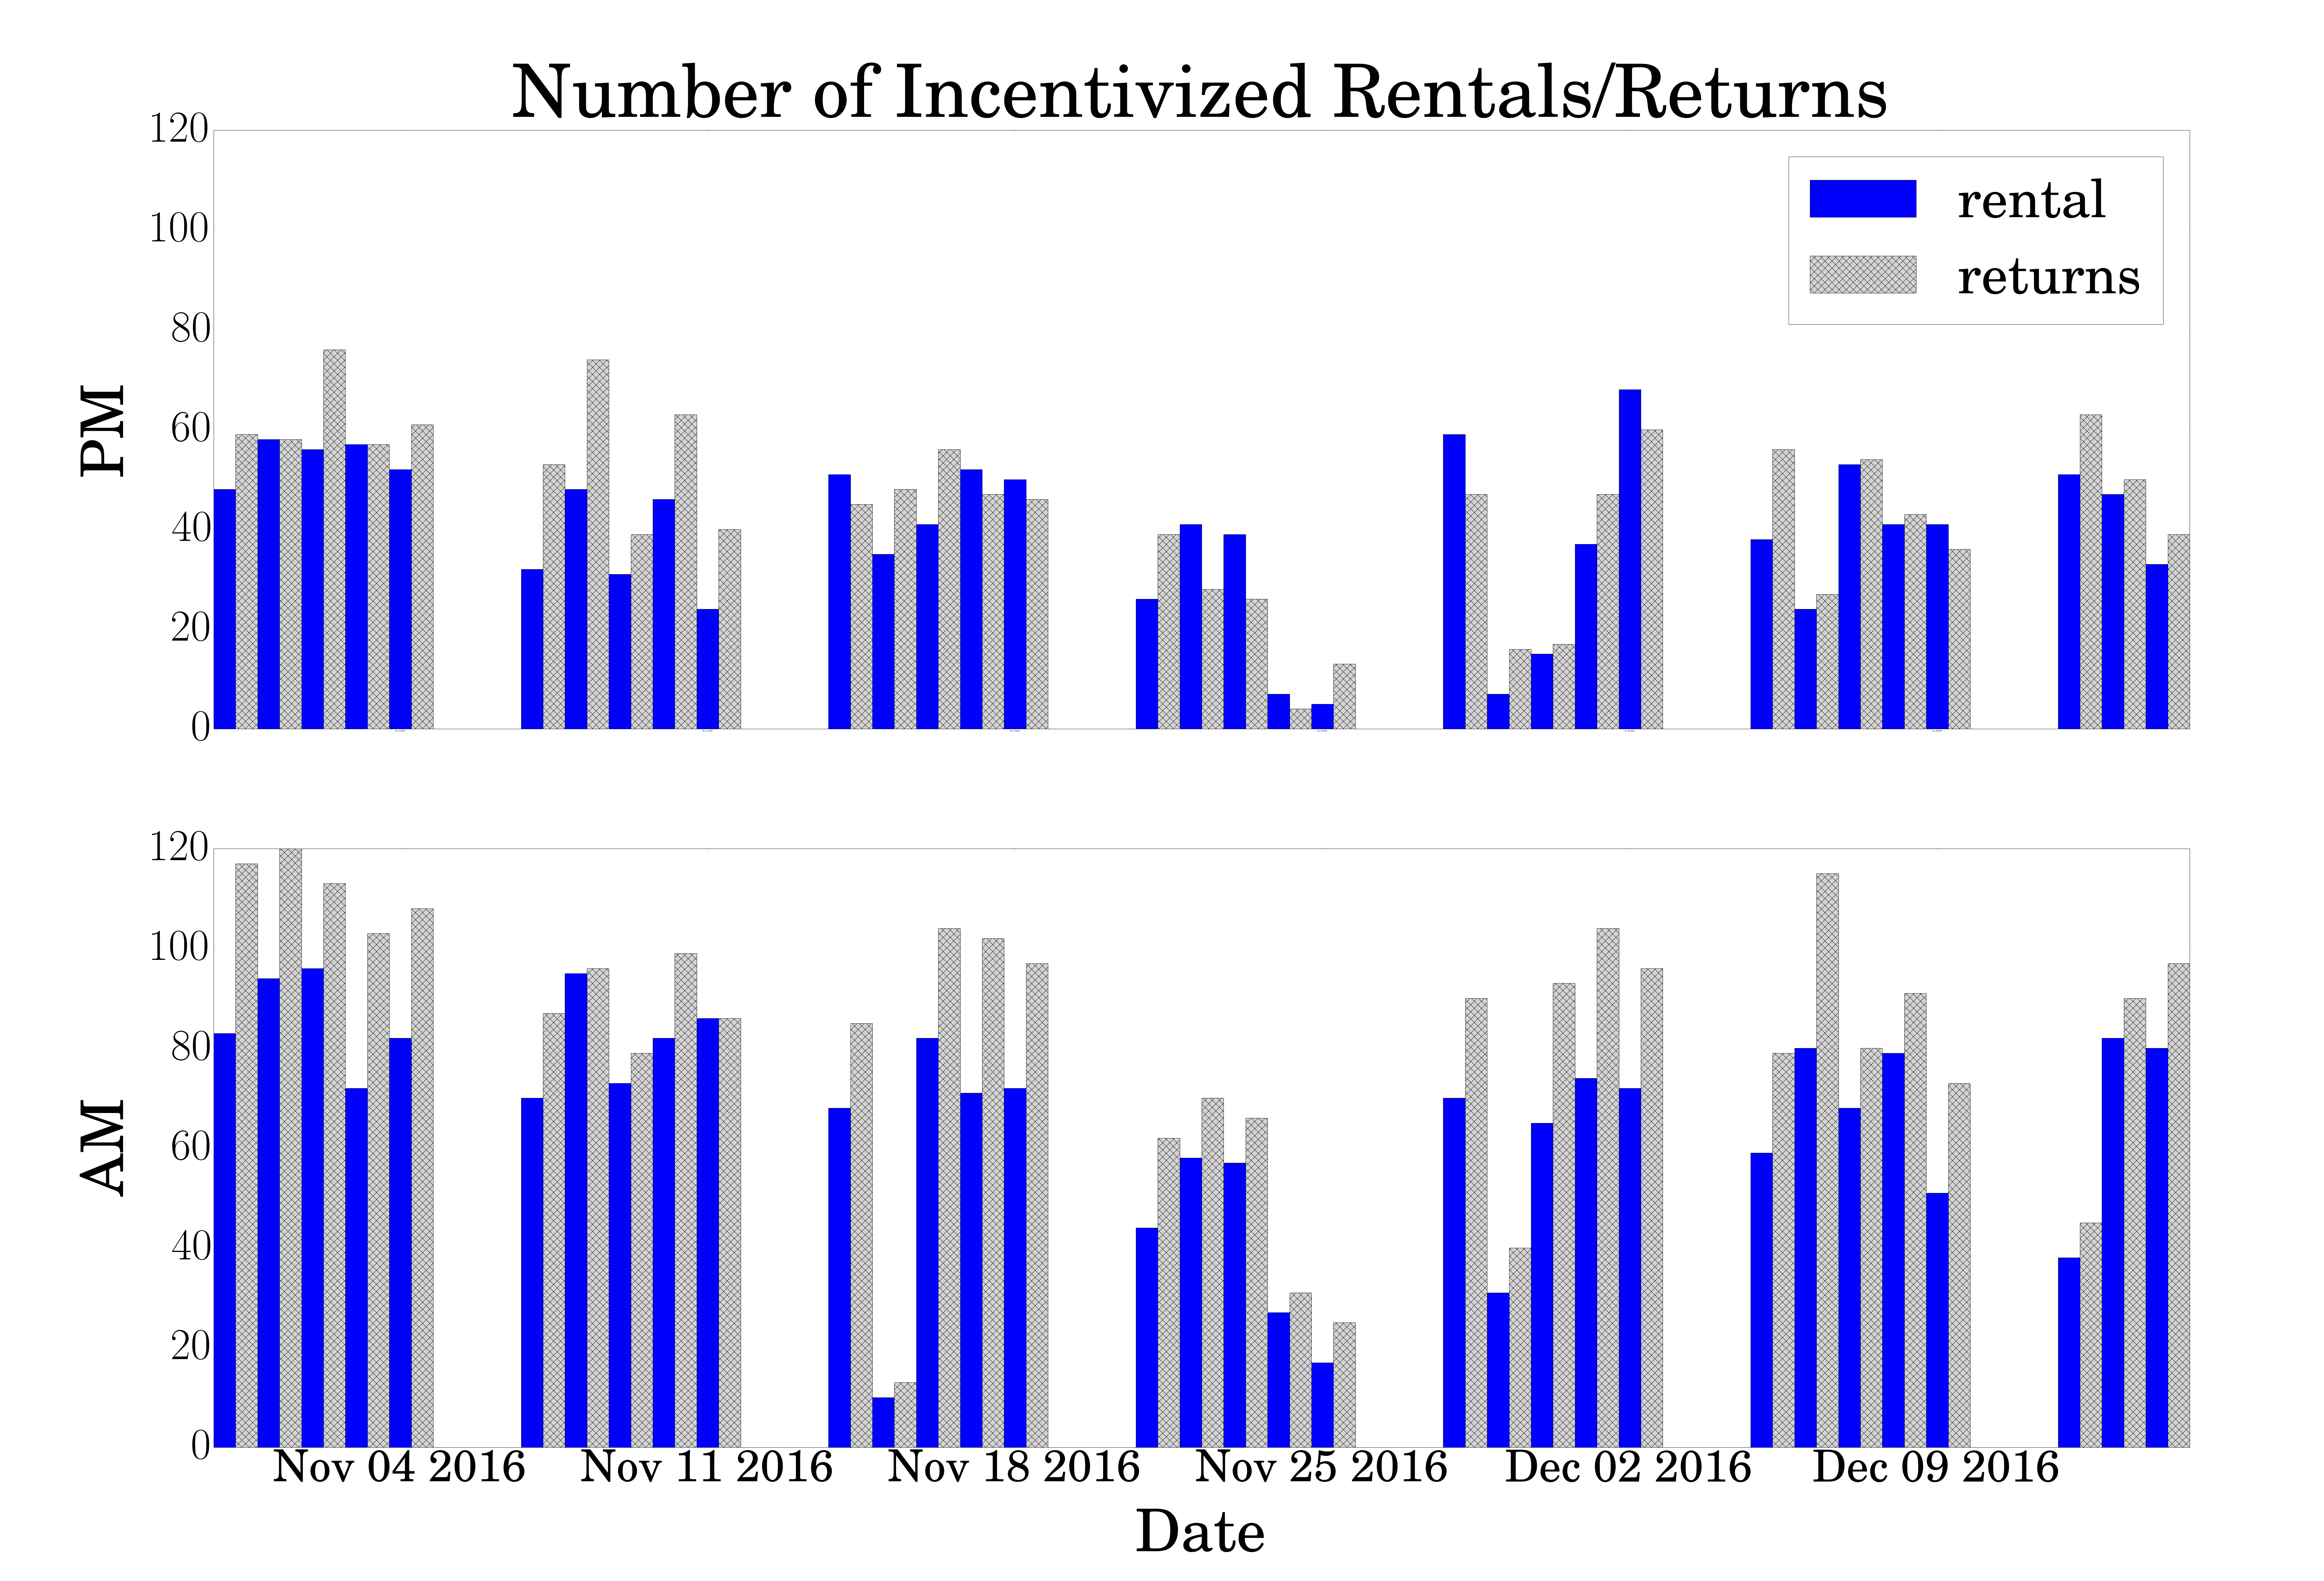
\includegraphics[width=.5\textwidth]{../SubmissionPlots/ActuallyUsed/Rental_Return.png}
\caption{Total number of incentivized rentals/returns in the test period.}
\label{fig:Incentivized Rentals/Returns}
\end{figure}

% While online policies thus h a downside with respect to The downside of such online decision making is the decreased perceived predictability of whether a (later) trip will be incentivized. The upside; however, is the increased efficiency of online policies as we will show in the next section. 	

\subsection{Offline Policies}

We first describe the offline policies. \emph{Offline} policies are characterized by the fact that the decision, for each AM/PM period, as to which interval will be incentivized for each station is made (irrevocably) at the beginning of that time interval (6AM and 4PM for AM and PM, respectively); in doing so, these policies have access to past data and the number of bikes at that time, i.e., 6AM and 4PM, respectively. %do not rely on 
(Note that this use of term offline is different from its use in other contexts, where offline often means that the algorithm has access to {\it all} of the data for the input to be optimized before needing to commit to any decision.) 

\subsubsection{Static}
The Static model is the simplest offline policy and was also the policy employed in Citi Bike at the time that this research project initiated. This policy determines a subset of stations to incentivize for which  the entire AM period is incentivized on every day, and similar subset is determined for the PM period. This model serves as a baseline against which all other policies are compared.

\subsubsection{Static Hindsight} 
The Static Hindsight model is an offline policy that chooses, for each station, the optimal continuous incentive period when looking back in hindsight for the past $q'$ weekdays. More precisely, the model assumes an incentive interval can start/stop every 30-minutes, starting from the beginning of the time period (e.g., 06:00 -- 07:30 or 07:00 -- 12:00 for the AM period), and chooses the incentive interval that achieves the highest performance when constrained on the past $q'$ weekdays of trip data. Throughout, we will use the term incentive interval to refer to such a continuous time period with these discrete start/end times. In our results, $q'$ is set to be 10. Thus, we let $D(d)$ denote the set of dates which are $q'$ days in hindsight;
we let $\tau(D(d), s)$ denote the possible morning incentive trips belonging to those dates and station $s$, and let $I_{d,s}$ to be the incentive interval for station $s$ on day $d$. Furthermore, let us say trip $r \in I$ if and only if the trip occurred during the interval $I$. The interval $I_{d,s}^\star$ chosen by Static Hindsight for the morning period is
\begin{equation}
\text{arg}\,\max\limits_{I}\ \sum_{r \in \tau(D(d), s)} \Delta_{r} \cdot 1_{r \in I} ,
\end{equation}
where the notation $1_{r \in I}$ means the indicator function that is equal to 1 if $r \in I$, and is 0, otherwise.

\subsubsection{Cluster Hindsight}
This offline policy uses a clustering of the stations to help make incentive decisions. As we describe in more detail below, the model first groups the stations by station dock-capacity, clusters each group by bike-level behavior, and finally chooses the optimal incentive interval for each cluster when looking back in hindsight (similar to Static Hindsight). 

We compute groups of stations by sorting them from smallest to largest capacity, and dividing them into $g$ roughly equal-size groups. %To be exact, we first group the stations into $g$ equal size groups, such that the smallest $\frac{1}{g}$ stations form the first group. 
The intuition for the grouping is our prior belief that station activity level is highly correlated with station capacity size and it is unwise, for example, to compare stations with bike-capacity 5 with stations of bike-capacity 60. The actual data-points used to cluster are 12-dimensional vectors consisting of the 12 half-hour interval bike-level percentages (bike-level divided by station dock capacity) for a station and date. The data points were obtained from our training data period, and bike-level percentages, rather than absolute values, were used to normalize the data points. To cluster each group of stations, we run the k-means clustering algorithm (k-centroids) with the objective of minimizing the distortion, which is defined to be the sum of the squared Euclidean distances between each vector and its centroid. Finally, our model uses a hard labeling system to associate each station with a single cluster (since for each station we have multiple points corresponding to distinct dates), and labels a station as belonging to the cluster for which its data points are most prevalent. 

To calculate the actual incentive intervals for each cluster, the model finds the optimal single, continuous incentive interval when looking back in hindsight of $q'$ weekdays for the stations in the cluster. Then let us define $C(s)$ to be the cluster of stations which $s$ belongs to. The interval that the model chooses is as follows:
\begin{equation}
I_{d,s}^\star= \text{arg}\,\max\limits_{I}\ \sum_{s' \in C(s)} \sum_{r \in \tau(D(d), s')} \Delta_{r} \cdot 1_{r \in I}
\end{equation}

The number of groups and the number of clusters are hyper-parameters of the model. To fit these parameters and avoid high bias/variance problems, k-fold cross-validation was used with our training data, and the parameters with the best average scores were chosen. Due to the temporal aspect of the data (e.g., weather plays a big role in system behavior) the k-folds were also divided to maintain the temporal order. The final parameters used in our results are $g$ = 10, $k$ = 3 and $q'$ = 10.

\subsubsection{Fluid Model}

A natural way to use the incentive-angel and non-angel rates to define an offline policy is by defining a so-called fluid model, in which it is assumed that exactly the expected number of rentals and returns occurs continuously per unit of time. Within such a model, it is easy to find the interval during which incentivizing minimizes the (fluid) number of out-of-stock events. In fact, one can show that under mild assumptions on the data, it is guaranteed that incentivizing over a single interval is optimal in such a model.

Though fluid models have successfully been applied to operational questions in bike-sharing, e.g., in \cite{jianetal}, we found in our analysis that the fluid model was vastly dominated by all other models; thus, we omit both its formal definition here and its performance in the results section.

\subsection{Offline Benchmark}

Offline policies are constrained in two ways: first, by the fact that we allow them to incentivize only during subintervals, as opposed to incentivizing, say, from 6-8AM and then again from 9-10AM but not in between; second, since the decision is based solely on the number of bikes at each station at 6AM, they lack information about demand later in the course of the day. To distinguish between the lack of information and the constraint of incentivizing only during a subinterval, we define the following \emph{static optimal} benchmark that has access to full information, but is constrained to incentivize only during a subinterval.

\subsubsection{Static Optimal}
The static optimal model is not a feasible policy since it assumes future knowledge that is not given in practice; instead, it is a model built in hindsight to benchmark offline policies. More specifically, for each week, station and AM/PM period, the Static Optimal model considers in hindsight, with complete knowledge, the best possible single continuous incentive period in which to incentivize.

\subsection{Online Policies}

In contrast to the offline policies described above, online policies gain information over the course of the day and thus are able to adopt whether or not to incentivize at a given station at a given time. We define only a very simple set of online policies.

\subsubsection{Dynamic}
The Dynamic model is a completely online policy that chooses in real-time for each trip whether or not it is incentivized to guarantee perfect efficiency. Formally, the model incentivizes all trips with $\Delta_r>0$ (cf. Equation 5), i.e., the performance is exactly the sum of all trips that contribute positively to the objective. This policy serves as an upper-bound on what any policy can possibly achieve within our analysis. 

\subsubsection{Dynamic CC (X)}
Beyond the fully dynamic model, we define a parameterized family of policies, wherein each policy breaks up the incentive period into intervals and the parameter X dictates the size of the intervals. For a given X, Dynamic CC starts at the beginning of each AM/PM period and decides every X minutes whether or not to incentivize trips for the next X minutes. To decide whether to incentivize the next X minutes, the model simulates the occurrence of one incentivized trip with the current number of bikes and empty docks at the station. If the simulated value of $\Delta_r$ is positive, Dynamic CC chooses to incentivize trips at the station for the next X minutes. For example, the Dynamic CC 15 model at 6 AM will check the station's current number of available bikes and docks, and simulate an incentivized trip for that user dissatisfaction function and that number of bikes and docks available. If the $\Delta_r$ value for this trip is positive, it will choose to incentivize the station from 06:00--06:15. Then, at 06:15 it simulates a new trip, based on updated information, to determine whether or not to incentivize from 06:15--06:30. 

We consider the Dynamic~CC policy for $X\in\{15,30,60,120\}$. Furthermore, one could also view the Dynamic model as Dynamic CC with $X=0$.

%Formally, for station $s$ and day $d$, let $t_x$ be the X-minute interval in question, $I(t_x)$ to be the binary incentive decision to incentivize or not, and $t$ be the half-hour interval to which $t_x$ belongs. Further, let $l_{s,t_x}$ be the bike-level at time $t_x$ and $\phi_{s,t}(l)$ be defined as in equation (??). Then $I(t_x)$ for arrival-incentives are calculated as follows: DOESN"T SEEM VERY PLEASING TO THE EYE. HOW SHOULD WE CHANGE THIS?
%\begin{equation}
%    I(t_x) = 
%    \begin{cases}
%      1  \{ \phi_{s,t}(l_{s,t_x}) - \phi_{s,t} (l_{s,t_x} + 1) - \beta \ge 0 \} & \text{ if deterministic} \\
%      1  \{ (\phi_{s,t}(l_{s,t_x}) - \phi_{s,t} (l_{s,t_x} + 1)) * p_{d,s,t} - \beta \ge 0 \} & \text{ if stochastic} \\
%    \end{cases}
%\end{equation} 




%\subsection{Fluid}
%The Fluid model is an offline policy that uses an estimation of the bike-level throughout the day to choose an incentive period which minimizes out-of-stock events. Given a potential incentive period as well as the starting bike-level at a station for the time period, the model uses the arrival/departure rates defined previously (c.f. equation (??)) to estimate the bike-levels after every 30-minute interval. Furthermore, if the estimated bike-level after a 30-minute interval is either below zero or above the dock-capacity of the station, the absolute quantity below zero or above the capacity can estimate the out-of-stock events occurring during the 30-minute interval. Thus to find the total estimated count of out-of-stock events occurring during the morning/afternoon period, the Fluid model estimates the fluid bike-level after each 30-minute interval, adds the interval's out-stock-events to the total count, and if necessary caps the bike-level below by zero and above by the dock-capacity, before moving onto the next 30-minute interval. 
%
%When considering the total estimated out-of-stock events, it is worthwhile to not only consider the out-of-stock events occurring during the period, but also the estimated future out-of-stock events from the resulting bike-level at the end of the period. The model incorporates this into its calculation by evaluating the user-dissatisfaction function at the estimated finishing bike-level and adding this to the total count. To find the best incentive period, the Fluid model chooses the incentive period which minimizes the total estimated out-of-stock events.
%
%Formally, let us define $f_{d,s,t}$ to be the expected bike-level for station $s$, on day $d$ and 30-minute time interval $t \in \{0, 1, 2,...,47\}$. Also for a station let $d_s$ be the dock-capacity, and $I$ be the incentive period indicating which 30-minute time intervals to incentivize. If the station is an arrival incentivized station for the morning period, $f_{d,s,t}$ can be calculated recursively as follows (similarly for afternoon and departure incentives):
%\begin{equation}
%    f_{d,s,t}=
%    \begin{cases}
%      \text{actual bike-level at 6 a.m.}, & t=12 \\
%      min(max(f_{d,s,t-1}, 0), d_s) + 30( \lambda_{d,s,t}^{r, +} +  \mu), & t \not\in I\\
%      min(max(f_{d,s,t-1}, 0), d_s) + 30(\lambda_{d,s,t}^{i, +} + \mu), & t \in I\\
%    \end{cases}
%\end{equation} 
%where
%\begin{equation}
%\mu =  - \lambda_{d,s,t}^{r, -} + \lambda_{d,s,t}^{n, +} - \lambda_{d,s,t}^{n, -}
%\end{equation}
%Finally, using the user-dissatisfaction function $\phi_{s,t} (l)$, the Fluid model chooses its optimal incentive period $I^*$ as such for the morning period (similarly for the afternoon):
%\begin{equation}
%I^*= \text{arg}\,\min\limits_{I}\  \phi_{s,24} (l) + \sum_{t=13}^{24} (0 - f_{d,s,t})^+ + (f_{d,s,t} - d_s)^+
%\end{equation}
%where
%\begin{equation}
%l = min(max(f_{d,s,24}, 0), d_s)
%\end{equation}



%
%
%\subsection{Offline/Online Decision Making}
%The different policies we analyze can be divided into two fundamental groups: offline and online policies. The offline policies choose, prior to the start of each morning/afternoon period,  a single continuous time period for which the station is incentivized. The motivation for a single continuous incentive interval is given by Proposition 1 and the performance of the Static Optimal, a static policy with perfect hindsight, shown later. Online policies, on the other hand, make dynamic decisions throughout the morning/afternoon periods and are not restricted to one continuous incentive interval. As we will see in the results section, that flexibility, combined with the additional information, makes the online policies more efficient. However, that improved efficiency comes at the cost of increased complexity and decreased perceived predictability for the user. 